\subsection{GyroScope and directional vectors}
Since one of the games required the player to build towers with the cubes and since project is about augmented reality, we thought it was a good idea to use the gyroscope rather than relying on the player to hold the phone the right way up. We also thought of using the gyroscope to separate four sides of interaction in the horizontal plane, but that is a compass and we couldn't expect the user to be facing north when playing the game. We could expect up to be up, but not west to be left, so for this we had to go with the unity-world-coordinates with the camera as center. The problem was just, how to use the gyroscope.\\
From a standard unity function we got the rotation of the real world from the gyroscope.The optimal thing to do would be to rotate the unity-world to be the same as this rotation. This however was not possible and the markers use global position so we couldn't make a virtual world object in unity to rotate.\\
We could have added the rotation to the cubes transforms, but we only needed to know the direction of collisions. So we made an object that rotates as the rotation from the gyroscope and that contains a child object thats local position is translated one unit up from parent object. This gives us a unit vector for the direction up in the real world.
\\
\begin{figure}[ht] 
        \capstart
        \centering  
        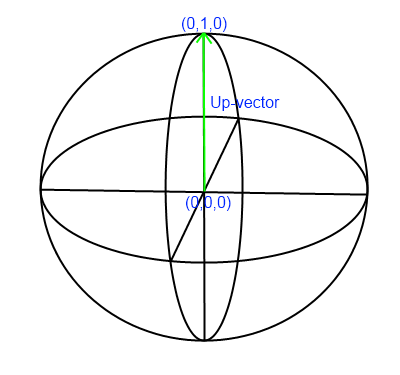
\includegraphics{images/GyroObjectModel.png}    
        \caption[Model of the game-object used to get the direction up]{Not the one we used in the application, but it illustrates the principle better without the extra functions. This object is fixed in the real world when the user rotates the device, so that the up-vector points up in the real world.} 
        \label{fig:Gyro_model} 
 Then on collision we can take the direction-vector between the colliding cubes. (cubeB.position - cubeA.position)
        \capstart
        \centering  
        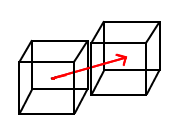
\includegraphics{images/CollisionDirectionObject.png}    
        \caption[Model of the collision direction vector]{The vector shows the direction from the cube in focus to the colliding cube.} 
        \label{fig:Collision_Direction_model} 
\end{figure}
\paragraph{Degree vertical}
By normalizing the vectors you can use the scalar product or dot product between the two vectors to find the vertical angle between the cubes.

\begin{figure}[ht] 
        \capstart
        \centering  
        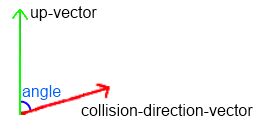
\includegraphics{images/CollisionDirectionAngleModel.png}    
        \caption[Model for finding the angle between the vectors]{The angle between the up-vector in the gyroscope-object and the collision-direction-vector from the cubes.} 
        \label{fig:Vector_Angle_model} 
        \capstart
        \centering  
        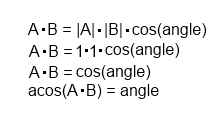
\includegraphics{images/AngleFormula.png}    
        \caption[Description]{A = collision-direction-vector, B = Up-vector, |x| = length of x, cos = cosine, acos = arc-cosine.} 
        \label{fig:Angle_Formula} 
\end{figure}

 The angle is 0-180 degrees. Less than 60 means one is below the other and more than 120 means one is above the other and if the angle is between 60 and 120, it's a horizontal collision. Having the gyroscope as an object in the scene was also very useful for visualization during testing.




